% Made up for the tikra gallery: a Lissajous figure, two oscillations at right angles.
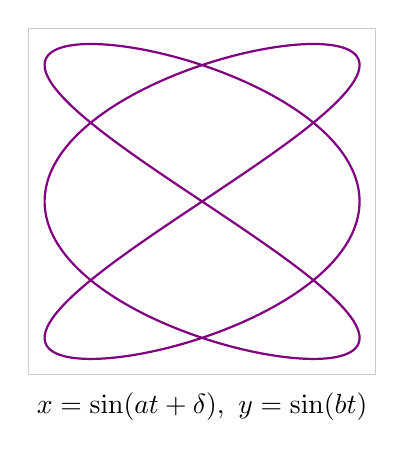
\begin{tikzpicture}
  \def\a{3}   % horizontal frequency, 1..7
  \def\b{2}   % vertical frequency, 1..7
  \def\d{90}  % the phase between them in degrees, 0..180
  \draw[gray!40] (-2.2,-2.2) rectangle (2.2,2.2);
  \draw[violet, thick, domain=0:360, samples=500, smooth] plot ({2*sin(\a*\x + \d)}, {2*sin(\b*\x)});
  \node[below] at (0,-2.3) {$x = \sin(at + \delta),\ y = \sin(bt)$};
\end{tikzpicture}
